%%%%%%%%%%%%%%%%%%%%%%%%%%%%%%%%%%%%%%%%%%%%%%%%%%%%%%%%%%%%%%%%%%%%%%%%%%%%%%%%%%%%%%%%%
% SECTION HYDRODYNAMIC SIMULATIONS 
%%%%%%%%%%%%%%%%%%%%%%%%%%%%%%%%%%%%%%%%%%%%%%%%%%%%%%%%%%%%%%%%%%%%%%%%%%%%%%%%%%%%%%%%%

\chapter{Hydrodynamic Simulations}
\section{2D Simulations}
\subsection{Simulations setup}
The physical setup used for our simulations is the so called "box in a star" method, meaning that we simulate some relatively very small internal region of a star. 

In our case for the 2D runs it will be a box of $2.50 \times 10^{9} \ \mathrm{cm}$ on the $x$ axis and $1.25 \times 10^{9} \ \mathrm{cm}$ on the $y$ axis. Gravity is constantly pointing downward on the $y$ axis with a magnitude of $1000 \mathrm{cm/s^2}$. This generates a pressure stratification in the fluid that covers approximately three pressure scale heights. 

The controlling parameter in our setup is the temperature gradient that can be initialized to any value. In our case we divided the simulated region in three parts. The bottom region (labeled as $1$) starts at the lower boundary and reaches $4/12$ of the domain, the central (labeled as $2$) proceeds until the middle, and the upper one (labeled as $3$) reaches the upper boundary, as shown in \ref{fig:tempprofile}. We define a parameter $\alpha_{i}$ ($i=1, 2, 3$) which is nothing but the fraction of the $\nabla$ over the $\nabla_{\mathrm{ad}}$. As seen in previous sections $\alpha_{i}<1$ implies stability in the $i-$region, instability otherwise. 

We always initialized the setup with $\alpha_{1} = \alpha_{3}$ widely smaller than $1$; and $\alpha_{2}=0.99$, which means a very precarious situation in terms of stability in the second region. A heating function furthermore heats the second region with a Gaussian profile (see \label{fig:tempprofile}) to generate convection that will expand downward and upward by entrainment. The values of $\alpha_{1}$ and $\alpha_{3}$ are controlling parameters for the bulk-Richardson number, since they are proportional to $\Delta b$. The advantage of simulating a strip of convection between two stable layers (miming a Shell convection) instead of a convective region at the bottom that grows upward (Core convection-like) is twofold: it gives us two convective boundaries to study instead of one, and we avoid high mach number at the boundary which can at times generate problems or unphysical situations. 

One of the hardest tasks has been to generate the correct amount of heating such that the turbulence standard deviation \textit{at the interface} was constant during the run (which is one of the ingredients of the bulk-Richardson number, hence one of the parameters we want to control in order to perform a differential study). In order to do that, the heating function is tuned such that, at $t=100K s$ the total heat generation is reduced to $50 \%$ of the original amount.

\begin{figure}[t]
\centering
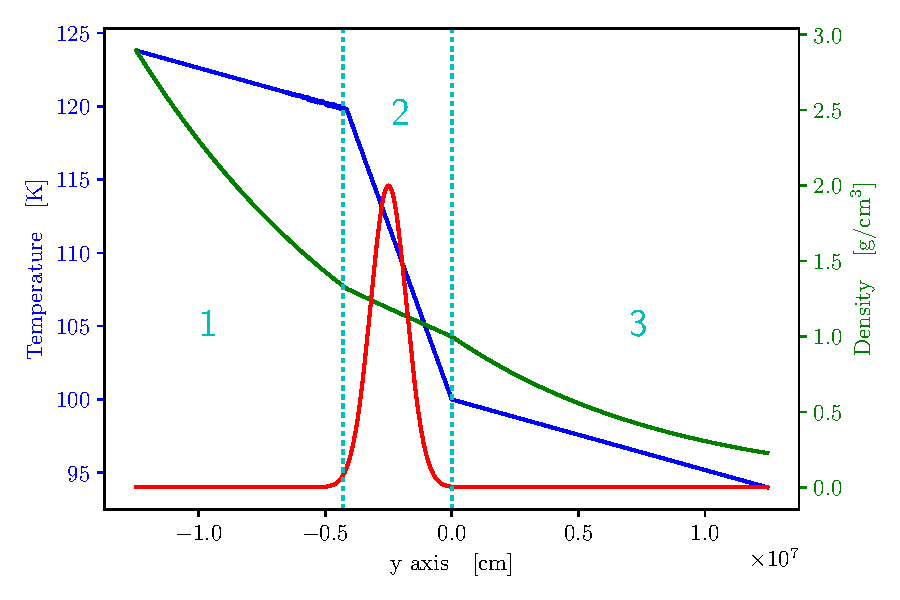
\includegraphics[width=10cm]{./img/twin.pdf}
\caption{Example of initial temperature profile along the $y$-axis}
\label{fig:tempprofile}
\centering
\end{figure}
At the bottom of the simulated region small perturbations in temperature and mach number had been imprinted on the stratification in order to break the initial symmetry of the system.

A wide range of boundary conditions have been tested for this problem. We used periodic boundaries for the horizontal direction, that definitely provide the most physical situation. For the vertical direction we used wall boundary conditions.

As briefly explained in the previous sections, in order to define the topology of the convective boundaries, we initialized a passive scalar inside each one of the regions. Recall that passive scalars are just like colors of the fluid and in no way influence the dynamics of the system, nor do they diffuse.

As previously stated our goal is to perform a \textit{differential} study of the bulk-Richardson number and the CBM problem. This implies running simulations with different values of $\Delta b$ and $\sigma_t$ at different resolutions. Being that 2D simulations computationally so cheap, we managed to run a copious amount of them. With the code 2d0.10-0.80 we will refer to a 2-dimensional run with $\alpha_{1} = \alpha_{3}=0.1$ and $80 \%$ of the heating referring to the arbitrary value of $4.5 10^{15} \mathrm{erg/s}$.

We run in 2D on a $2048 \times 1024$ uniform Cartesian grid. It is worth remarking that when doing CFD with a higher resolution, one not only better resolves the features of the system, but also decreases the numerical viscosity (increases the Reynolds number). This is the reason for which we chose this grid setup: we want to keep cells squared and keep viscosity a scalar quantity, and prevent it from becoming a tensorial one. In the next section we will perform a convergence study, in order to understand which roles the resolution and the viscosity play in the phenomenon of convective entrainment.


\subsection{Evolution of a single run}



\begin{figure}[t]
      \centering
        \subfloat[Mach number profile over time.]{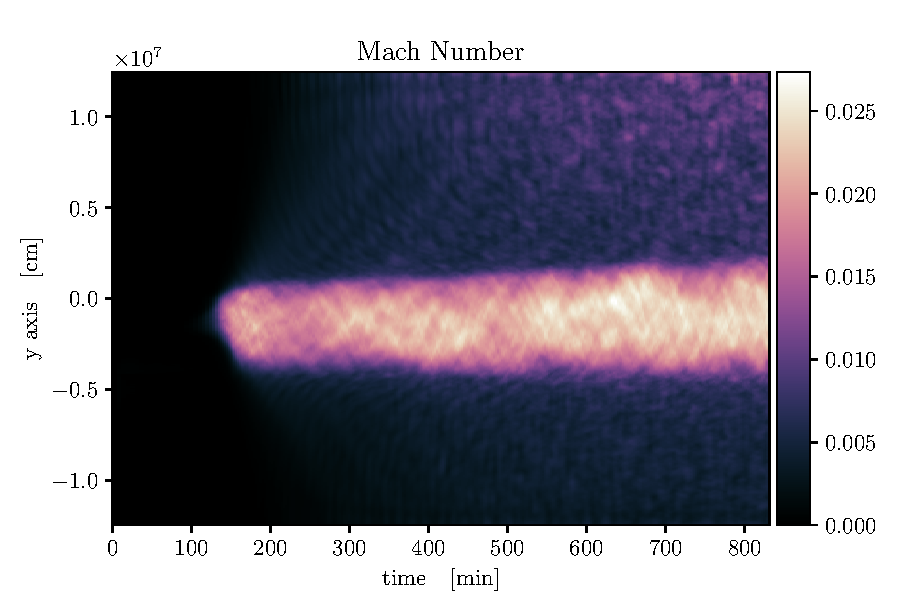
\includegraphics[width=9.9cm]{./img/mach.pdf}\label{fig:2d0.7-0.01LR.turbmach}}
     \centering
	\hfill
        \subfloat[Entrainment of passive scalar from the upper stable region in the convective region.]{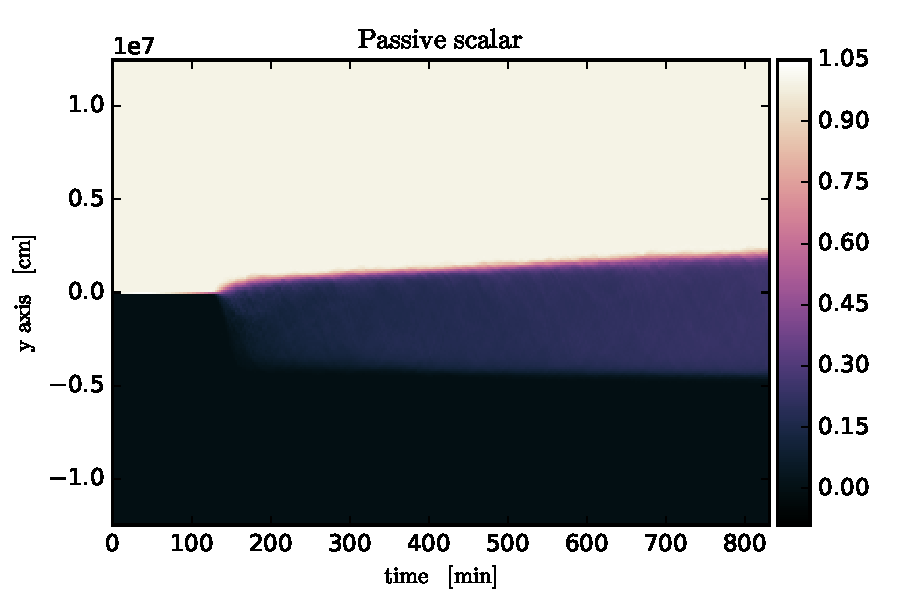
\includegraphics[width=9.9cm]{./img/ps2.pdf}\label{fig:2d0.7-0.01LR.bp}}
	\caption{Time evolution of a 2D run.}
	\label{2dsingle}
\end{figure}
 %%%%%%%
 % divisione figure %
 %%%%%%%

Let's consider the setup 2d0.10-0.80. 

Convection starts at around $t \sim 7000 s$. Because of the already mentioned implicit time stepping, the lower the mach number, the bigger the time step, allowing us to save a huge amount of computational resources before the rise of convection. A remarkable difference is also observed in the convective regime, as long as the mach number is below $10 \%$, which has always been our case.

In figure \ref{fig:2dsingle} we plot the profile of the mach number over the simulated time. This is what one would expect, with two remarks that need to be done. 

First of all the mach number is stable over time, thanks to the heating function that we implemented, featuring a decrease of heat generation as previously explained. 

Second of all it is clear that some internal modes are excited by the convective blobs when they hit the stable layers and they propagate through it. They appear more significant in the upper region and to a certain extent it's true, but mainly this is due to the fact that the speed of sound there is lower. The difference is not so dramatic when plotting the absolute velocity. Two interesting questions remain without answer. First of all it is impossible to tell to which extent the dynamic of the boundary is influenced by these modes. Second of all it is possible that the chemical mixing due to these modes in the stable stratification might have a significant impact on the evolution of a star, which is obviously not considered in 1-D simulations.

\begin{figure}[t!]
  \centering
  \subfloat[Passive scalar avection at the onset of convective motions, at $t \simeq 150 \ \mathrm{min}$]{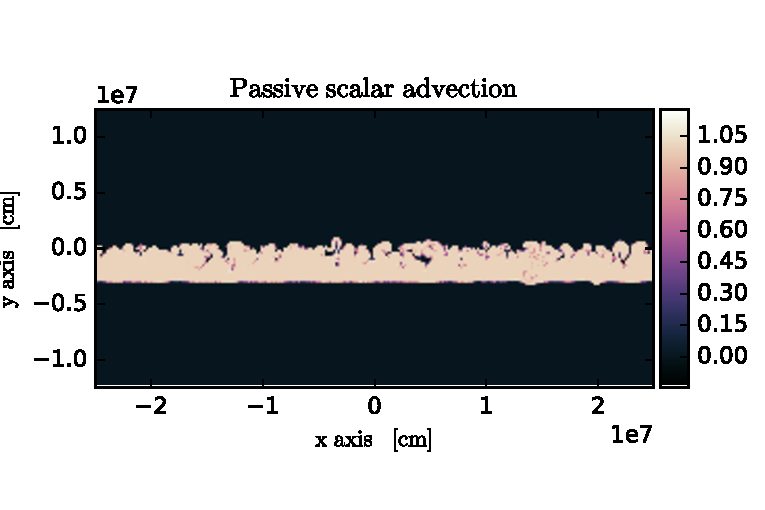
\includegraphics[width=10cm]{./img/passiveacc1.pdf}\label{fig:bulk}}
  \centering
  \hfill
  \subfloat[The same passive scalar of above, advected at $t \simeq 800 \ \mathrm{min}$. This defines the topology of the boundary.]{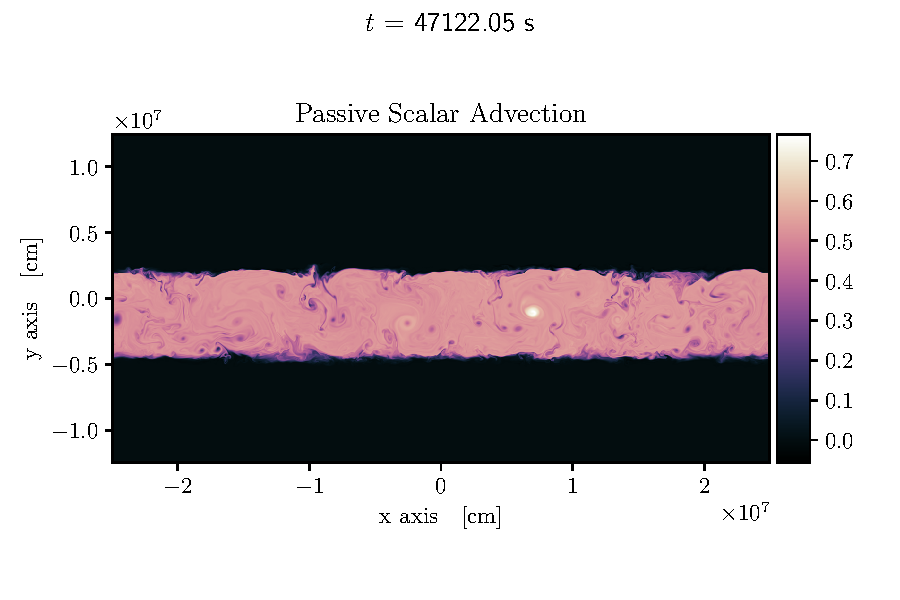
\includegraphics[width=10cm]{./img/passiveacc2.pdf}\label{fig:ent}}
  \end{figure}
  In figure \ref{fig:2dsingle} we plot the passive scalar initialized inside the upper region, which over time is entrained by convection. We clearly see the movement of the boundaries that over the $800 \ \mathrm{min}$ of simulated time move gradually upward and downward. Specifically in the upper case it starts in the middle of the simulated region and ends up at $\sim 7.0 \times 10^{6} \ \mathrm{cm}$, for the lower case it starts at $\sim 3.7 \times 10^{6} \ \mathrm{cm}$ and moves downwards to the middle of the simulated region 

In figure \ref{fig:2dsingle} we plot some parameters relevant to our analysis. 

\begin{figure}[t!]
  \centering
    \subfloat[Bulk-Richardson number over time.]{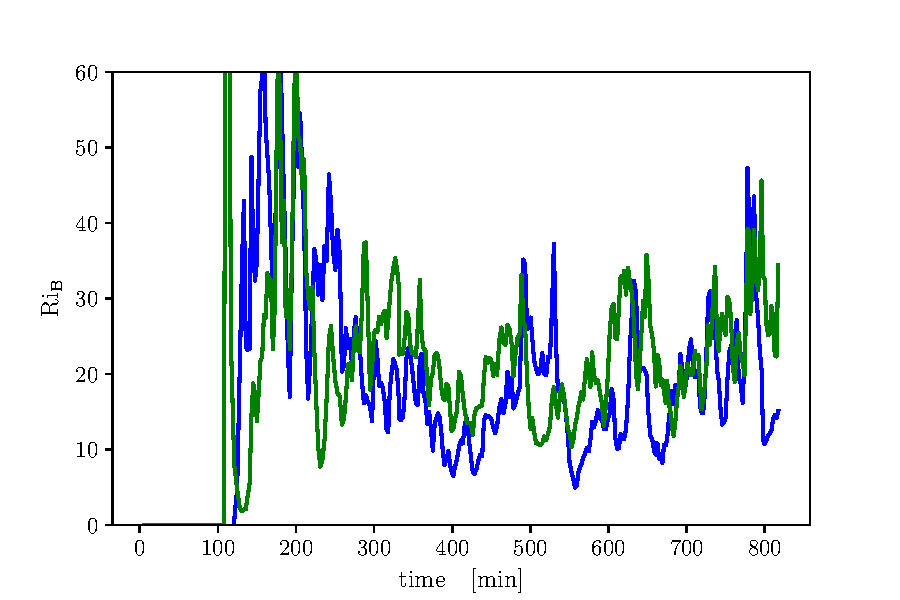
\includegraphics[width=0.5\textwidth]{./img/bulk.pdf}\label{fig:bulk}}
      \hfill
        \subfloat[Entrained mass over time.]{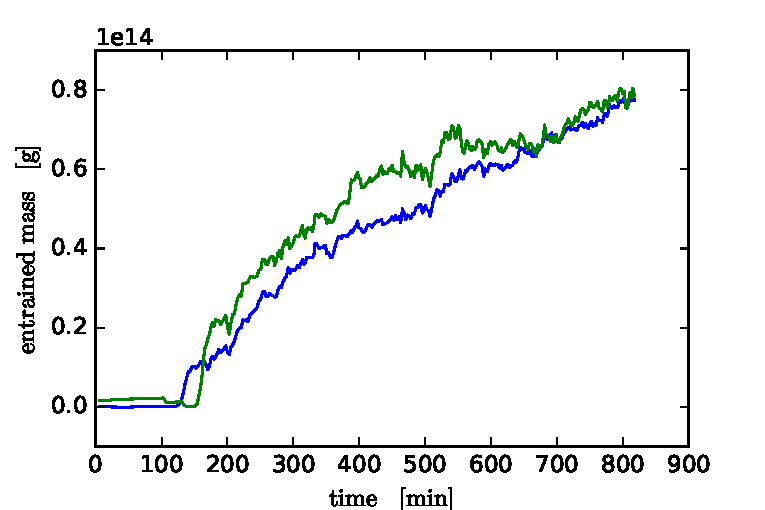
\includegraphics[width=0.5\textwidth]{./img/ent.pdf}\label{fig:ent}}
	\hfill
  \centering
    \subfloat[Turbulence standard deviation over time.]{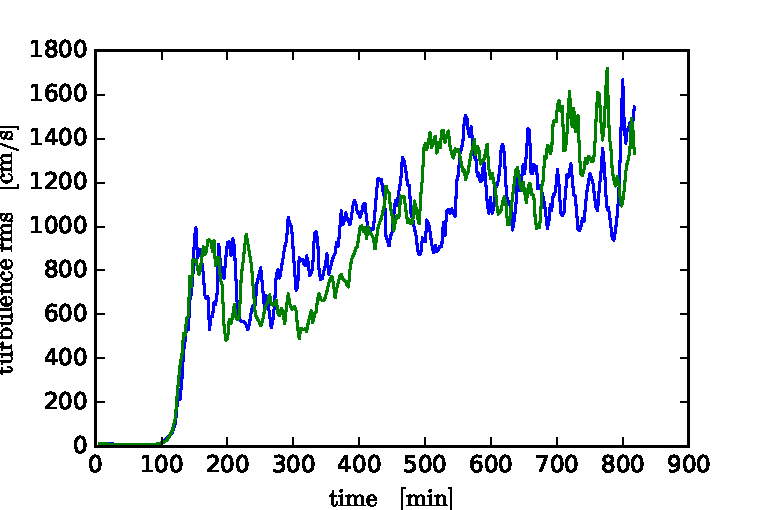
\includegraphics[width=0.5\textwidth]{./img/sigt.pdf}\label{fig:sigt}}
      \hfill
        \subfloat[Turbulence length scale over time.]{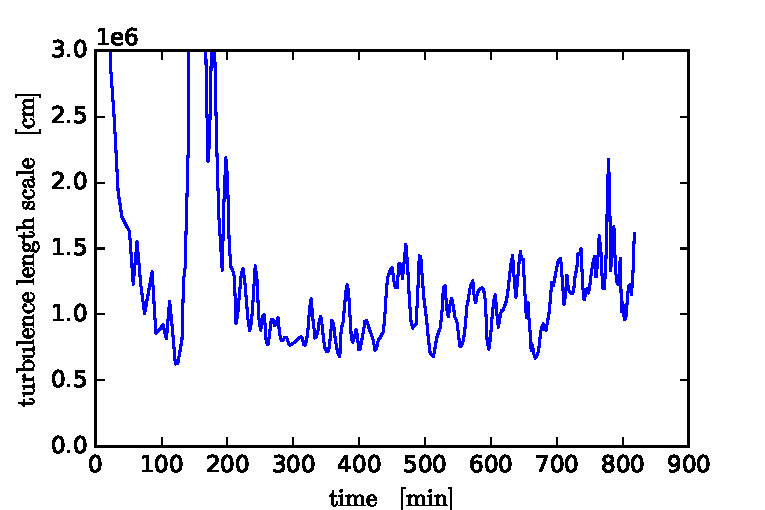
\includegraphics[width=0.5\textwidth]{./img/len.pdf}\label{fig:len}}
	\hfill
  \centering
    \subfloat[Buoyancy jump over time.]{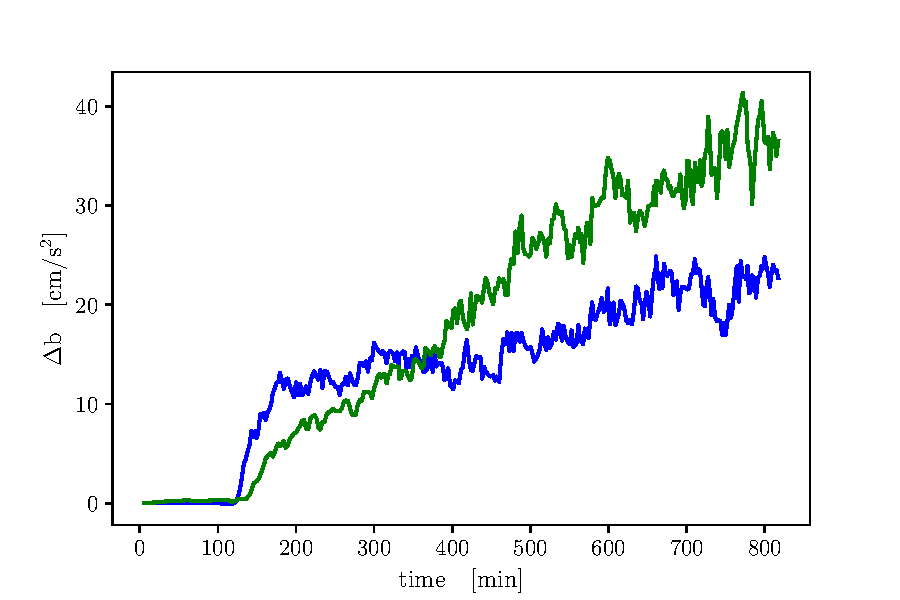
\includegraphics[width=0.5\textwidth]{./img/delb.pdf}\label{fig:delb}}
      \hfill
        \subfloat[Bounday position and width over time. Shaded regions represent the boundary thickness.]{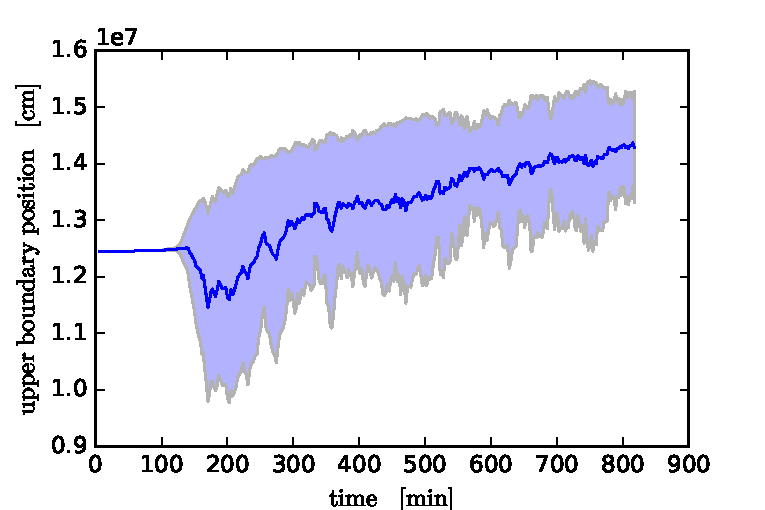
\includegraphics[width=0.5\textwidth]{./img/boundpos.pdf}\label{fig:boundpos}}
	\caption{Plots of the relevant parameters for our analysis over time. Blue lines represent the upper boundary, green lines the lower boundary.}
	  \label{fig:2dsingle}
  \end{figure}
We show first of all the bulk-Richardson number over time. Blue lines represent the upper boundary, green lines lower boundary. At around $t=\mathrm{300 \ min}$, when the entrainment becomes linear, the bulk-Richardson number still oscillates over half an order of magnitude. This obviously deeply affects our data analysis, making necessary a large amount of runs to collect as much data as possible. This also makes a differential study of the entrainment over time impracticable. 

Second of all we plot in figure \ref{fig:ent} the entrained mass over time. As already mentioned we will perform a Lagrangian study of entrainment, because it is impracticable to quantify how much of the boundary movement is due to the entrained mass or to the adiabatic expansion of the fluid. We notice that also the entrainment rate stabilizes after the initial transition. 

  In figure \ref{fig:sigt} we plot the turbulence standard deviation over time. It is overall constant, with a slight trend to increase. This result has been obtained after extensive tests to correctly tune the heating function.

  In figure \ref{fig:len} we plot the turbulent length scale $L$ over time. In this case we only calculated $L$ at the center of the convective layer, so this value will be used both for the upper and lower boundary analysis. The length scale at the interfaces has a value which is overall comparable, but it is affected by some spikes, reason for which we decided to calculate it in a fully convective region.

  The last ingredient of the bulk-Richardson number is the buoyancy jump $\Delta b$, that we plot in figure \ref{fig:delb}. In both cases there is an increasing trend, more significant in the lower boundary. This plot shows one of the biggest challenges of running simulations to study differentially the bulk-Richardson number: it is extremely hard to obtain a run where all the parameters ($\Delta b$, $L$, $\sigma_t$ and $M_{\mathrm{E}}$) are constant over time. Hence one finds itself in the inconvenient situation of having to average over values that span a full order of magnitude with a strong increasing or decreasing trend, and the quality of the analysis is consequentially affected by this uncertainty.

 \begin{figure}[t!]
\centering
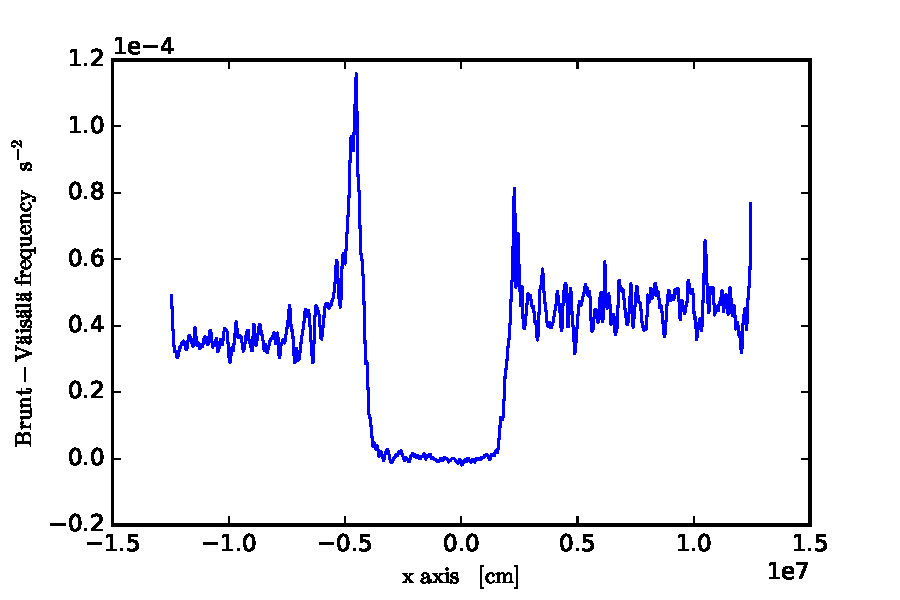
\includegraphics[width=0.6\textwidth]{./img/brunt}
\caption{Horizontal average of the Brunt-Väisälä frequency at about $t=500 \ \mathrm{min}$.}
\label{fig:brunt}
\centering
\end{figure}
For completeness we plot the boundary position over time in \ref{fig:boundpos.pdf} As previously mentioned an Eulerian study is impracticable for this phenomenon, because it is hard to quantify how much of the boundary migration in an Eulerian frame is due to the entrainment and how much due to the adiabatic expansion of the fluid. Nevertheless we would like to point out that, once the entrainment rate stabilizes at $t=300 \ \mathrm{min}$, the boundary thickness is also overall stable in both the upper and lower case. 

For every 2D or 3D run we will extrapolate the relevant parameters and present them in the following layout
\begin{center}
 \begin{tabular}{l|c|c}
	 Run &2d0.7-0.01U&2d0.7-0.01L\\
	  	\hline
	   $\Delta b$ $(\mathrm{cm/s^{2}})$&$ 18.17 \pm 3.62 $&$27.68 \pm 7.18$\\
		\hline
	   $\sigma_t$ $(\mathrm{cm/s})$ &$ 1118 \pm 202 $&$1190 \pm 218$\\
		\hline
	   $L$ $(\mathrm{cm})$&$(10.88 \pm 2.56) \times 10^5$&$(10.88 \pm 2.56) \times 10^5$\\
		\hline
	   $Ri_{\mathrm{B}}$& $17.070 \pm 7.407 $&$21.622 \pm 6.538$\\
		\hline
	   $\dot{M}_{\mathrm{E}}$ $(\mathrm{g/s})$ &$(1.287 \pm 0.006) \times 10^9$&$(9.125 \pm 0.015) \times 10^8$\\
      \end{tabular}
 \end{center}
 Where the U at the end of the run name stands for upper boundary, and the L for lower boundary. 

 Notice that the lower boundary is stiffer than the upper one (the buoyancy jump is higher, and hence the bulk-Richardson number) even if in the initial setup the Brunt-Väisälä frequency is the same for the two stable regions. Looking at figure \ref{fig:brunt} it is clear that at the convective boundaries a spike arises during the simulation in the Brunt-Väisälä frequency, and in the lower case it is more pronounced. Obviously when integrated over the interface, this gives rise to a bigger buoyancy jump. These spikes in the Brunt-Väisälä frequency at the interfaces were also found by Arnett \emph{et al.} (2015).


\subsection{Resolution study}
\begin{figure}[t!]
  \centering
  \subfloat[Mach number profile for the $2048 \times 1024$ run.]{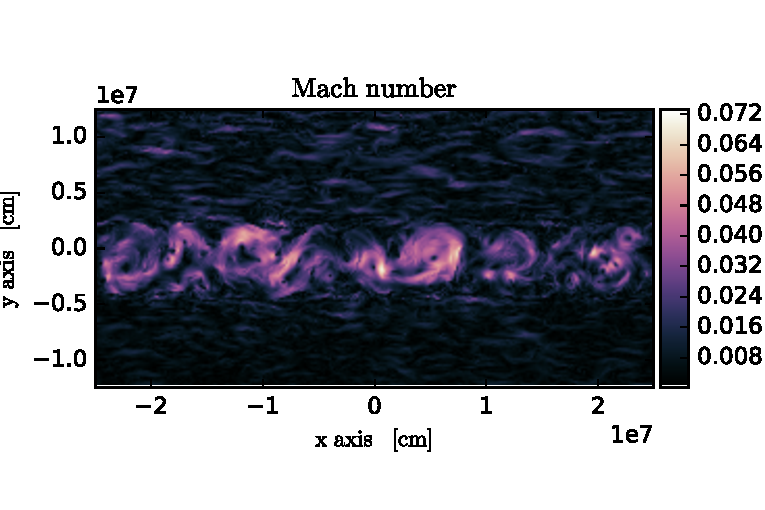
\includegraphics[width=10cm]{./img/machhighres.pdf}}
  \centering
      \hfill
    \subfloat[Mach number profile for the $512 \times 256$ run.]{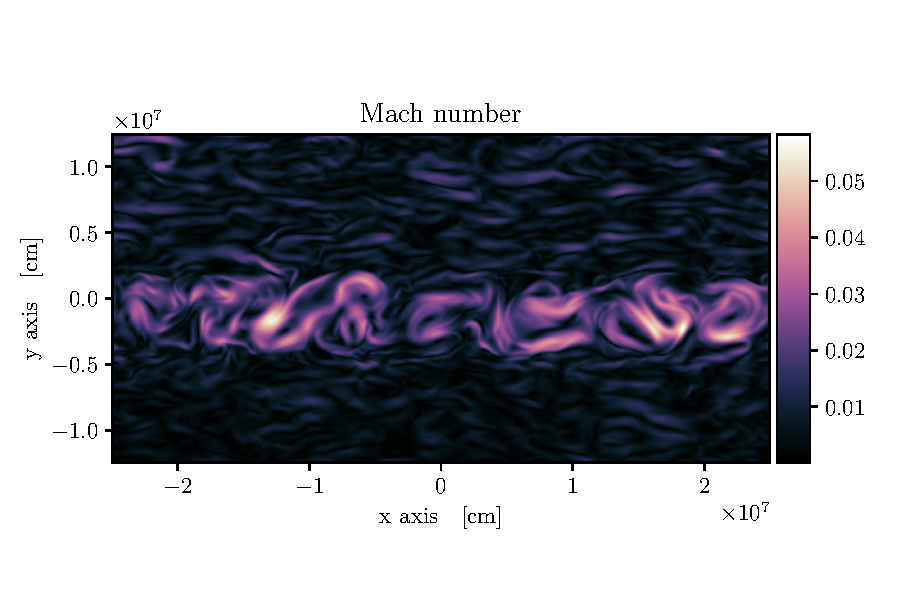
\includegraphics[width=10cm]{./img/machlowres.pdf}}
    \caption{Turbulent structures at different resolutions at about $t=500 \ \mathrm{min}$.}
    \label{fig:differentialmach}
 \end{figure}
In the last section we analysed the run 2d0.10-0.80. What we will do in this section is to compare the previous results with the ones obtained by running the same setup on smaller resolutions, in order to understand if we are properly resolving the system. 

The same setup was run on a $1024 \times 512$ and $512 \times 256$. As expected, the highest resolution run shows smaller and more refined turbulent structures in the convective region, while in the smallest run we observe less eddies but of bigger size (see figure \ref{fig:differentialmach}).

We report in the following table the relevant parameters of the upper boundary for the different resolution runs. We observe that all the parameters are overall constant, within a $10 \%$ oscillation range. Woodward \textit{et al.} (2016) found that the entrainment rate decreases exponentially with the enhancement of the resolution, before converging to the physical value. In our case we observe a constant entrainment (with a slight increasing trend, we presume due to second order phenomena), hence we can safely assume that even in the lowest resolution case we are properly resolving the system. Notice that the turbulence standard deviation increases with the resolution as expected, because of the higher Reynolds number due to smaller numerical viscosity. 

One could still point out that the convergence reached in a 2D setup does not imply a convergence in 3D, but being that 3D simulations are computationally so expensive, it is impracticable for us to test this hypothesis.
\begin{center}
 \begin{tabular}{l|c|c|c}
	 Run &$2048 \times 1024$ U& $1024  \times 512$ U& $512 \times 256$ U\\
	  	\hline
		$\Delta b$ $(\mathrm{cm/s^{2}})$ & $ 18.17 \pm 7.41 $ & $15.48 \pm 2.31$ & $12.82 \pm 2.40$\\
		\hline
		$\sigma_t$ $(\mathrm{cm/s})$ & $ 1118 \pm 202 $ & $1020 \pm 196$ & $970 \pm 233$\\
		\hline
		$L$ $(\mathrm{cm})$&$(10.88 \pm 2.56) \times 10^5$ & $(11.07 \pm 3.30) \times 10^5$ & $(11.50 \pm 1.71) \times 10^5$\\
		\hline
		$Ri_{\mathrm{B}}$& $17.070 \pm 7.407 $ & $17.694 \pm 8.397 $ & $17.598 \pm 7.663$\\
		\hline
		$\dot{M}_{\mathrm{E}}$ $(\mathrm{g/s})$ &$(1.287 \pm 0.006) \times 10^9$&$(1.255 \pm 0.013) \times 10^9$ & $(1.174 \pm 0.016) \times 10^9$\\
      \end{tabular}
 \end{center}
Even at the lower boundary all the parameters oscillate within a $10 \%$ range. The only exception is the bulk-Richardson number but this is affected by a significant error in the lower runs. Again in the higher resolution case the turbulence standard deviation is higher, as the entrainment rate.
\begin{center}
 \begin{tabular}{l|c|c|c}
	 Run &$2048 \times 1024$ L& $1024  \times 512$ L& $512 \times 256$ L\\
	  	\hline
		$\Delta b$ $(\mathrm{cm/s^{2}})$ & $ 27.62 \pm 6.54 $ & $25.85 \pm 6.48$ & $25.46 \pm 6.15$\\
		\hline
		$\sigma_t$ $(\mathrm{cm/s})$ & $ 1190 \pm 202 $ & $985 \pm 179$ & $977 \pm 143$\\
		\hline
		$L$ $(\mathrm{cm})$&$(10.88 \pm 2.56) \times 10^5$ & $(11.07 \pm 3.31) \times 10^5$ & $(11.50 \pm 1.71) \times 10^5$\\
		\hline
		$Ri_{\mathrm{B}}$& $21.622 \pm 6.538 $ & $31.934 \pm 17.718 $ & $33.334 \pm 17.721$\\
		\hline
		$\dot{M}_{\mathrm{E}}$ $(\mathrm{g/s})$ &$(9.252 \pm 0.015) \times 10^8$&$(1.006 \pm 0.017) \times 10^9$ & $(1.026 \pm 0.031) \times 10^9$\\
      \end{tabular}
 \end{center}




\subsection{Differential 2D study}

\section{3D simulations}

\subsection{Evolution of a 3D run}

\subsection{Differential 3D study}
